\chapter{Statistics of China's ``South Flood-North Drought'' Pattern and Associated Jet Changes}

\section{to-do}
1) May have to check how much Wang2013 beat you to the punch;

\section{Does the ``South Flood-North Drought'' reflect a jet shift?}

	We also explore decadal changes in the subtropical jet, which plays an essential and complex role in East Asian climate both in summer and winter \citep{Molnar2010,Yang2002}. In a region of strong fronts as observed in East Asia, theory predicts that the core of maximum zonal wind should anchor an equatorward region of ascent and strong rainfall \citep{Holton2004}. The Tibetan Plateau couples with the jet nonlinearly, amplifying the regional response to global climate anomalies \citep{Nigam1989,Broccoli1992,Park1997}. The jet's passage north of the Tibetan Plateau in summer is argued to dictate the timing of onset of the Indian and East Asian monsoons, both in present-day \citep{Yin1949,Yeh1959,Hahn1975} and on paleoclimate timescales \citep{Nagashima2011,Nagashima2013,Chiang2015}. On a weekly timescale, the jet serves as a waveguide for storms propagating from the Eurasian interior via the ``Silk Road'' teleconnection \citep{Hoskins1993,Ambrizzi1997,Kosaka2012}, and shifts in its latitude and strength induce corresponding rainfall anomalies \citep{Liang1998,Kwon2007,Du2009,Li2014}. Thus, we expect that the South Flood-North Drought has also entailed \nth{20}-century changes in the East Asian tropospheric jet. Therefore, we compare our rainband database to a database of jet counts from 1958 to 2001 from \citet{Schiemann2009} in search of coupled change.
	
\subsection{Jet Count Density} 

	\citet{Schiemann2009} constructed a data set of jet `counts' in the Tibetan Plateau region (46$^{\circ}$ E-130$^{\circ}$ E, 17$^{\circ}$ N-58$^{\circ}$ N) from ERA-40 reanalysis for 1958-2001, where a count is defined as any local maximum in zonal wind with westerly magnitude greater than $30$ m s$^{-1}$; further details can be found in section 2 of \citet{Schiemann2009}. We show daily mean jet latitude averaged across $90-130^\circ$E in Figure ~\ref{fig:jet_seasonal}a and monthly anomalies in Figure ~\ref{fig:jet_seasonal}b. Results are not sensitive to the choice of longitude range. Figure ~\ref{fig:climo} presents contours of jet frequency estimated by a kernel density method, which estimates a probability distribution from a set of discrete data observations.

\subsection{Dynamics}

	The tropospheric jet marks the northern boundary of the Hadley Cell, and shifts in response to seasonal changes in insolation \citep{Bordoni2008}. Beginning in May, the East Asian jet moves from its winter position on the southern flank of the Tibetan Plateau to a summer latitude well north of the plateau. During this transition, the jet occupies intermediate configurations that correspond to different stages of China rainfall (Figure ~\ref{fig:climo}). A full monthly jet climatology is visible in \citet{Schiemann2009}. Peak rainfall rates in China from May to mid-July corresponds to the months when the climatological latitude of the jet impinges on the Tibetan Plateau. The interaction of the tropospheric jet and Tibetan Plateau strengthens convergence and rainfall downstream over China and the western Pacific Ocean \citep{Molnar2010,Sampe2010,Chen2014}. From May to September,  the climatological latitude of rainfall, rainbands and jet density are all closely coupled, with peak jet density occurring 5 to 10 degrees north of the latitude of peak rainfall. The initiation of the Pre-Meiyu corresponds roughly to the beginning of the jet's northward passage. During Meiyu season, the preferred latitude of the jet continues to shift northward. The period of frequent double rainband occurrence during the Post-Meiyu corresponds to the jet's maximal northward extent. Finally, the jet returns southward during the Fall Rains in October and November, which produces only a weak rainfall response.
	
	In addition, Figures ~\ref{fig:climo}a-e show mean rainfall, jet frequency and rainband position during each stage, as well as their zonal average (sidebars). From the Pre-Meiyu to Post-Meiyu, each northward jump in peak rainband frequency corresponds to a similar shift in jet count density, with a southward offset of about 5 degrees.
	
\subsection{Jet Changes, 1980-2001 Versus 1958-1979}

	In Figure ~\ref{fig:jet_seasonal}a, we show the zonal average over $90-130^\circ$E) of mean jet latitude, averaged over the years 1958-1979 (blue solid line) and 1980-2001 (dashed red line) with 95\% confidence intervals overlain. Both significant changes in rainband statistics described in the previous section correspond to southward shifts in mean jet latitude. During the Pre-Meiyu (May), the tropospheric jet is shifted southward by almost 2$^{\circ}$ in 1980-2001 relative to 1958-1979, when its mean latitude was $\approx 41^{\circ}$N. We estimate the significance of this change using a two-tailed Kolmogorov-Smirnov (K-S) test. Since the K-S test requires that all samples are independent, we first remove temporal autocorrelation due to synoptic variability by assimilating daily mean jet latitude into 4 day blocks. A subsequent K-S test finds that the shift is significant with $p=0.003998$. During the Post-Meiyu (days 201-273), when a southward shift in rainband latitude is found in 1980-2001 relative to 1958-1979, the mean latitude of the jet is also consistently displaced southward. We assimilate daily mean jet latitude into 7-day blocks before performing a K-S test, and find a $p$-value of this shift of $p=0.05667$.
	
\section{Hypothesis}

	The Meiyu front and tropospheric jet covary in latitude from May to September in the climatological mean, and parallel changes are found in rainband attributes and mean jet latitude between 1951-1979 and 1980-2007. Therefore, the South Flood-North Drought appears to reflect an alteration in jet dynamics. We propose that both the Pre-Meiyu decline in rainband frequency and the Post-Meiyu southward shift of rainband latitude result from a single phenomenon: an overall southward displacement of the jet's summer progression over East Asia. In climatology, the Pre-Meiyu corresponds to both a surge in rainfall and the beginning of the jet's northward transit, when its preferred latitude begins to impinge on the Tibetan Plateau. We propose that the observed southward shift in the jet during May has delayed the date when the jet first impinges on the Tibetan Plateau, resulting in a delay in Pre-Meiyu onset and prolonged Spring Rain conditions. This is manifested as weaker rainfall and decreased rainband frequency in central China in May. Subsequently, we argue that the reduced northward extent of the jet during the Post-Meiyu has shifted rainfall and mean rainband latitude southward. Finally, we suggest that the southward displacement of the summer jet cycle results in a decrease in northern China annual rainfall and an increase in central China annual rainfall, producing a South Flood-North Drought response. Thus, our hypothesis can explain the major observed changes in rainfall and rainband statistics during the Pre- and Post-Meiyu as well as cumulative yearly change.
	
	To test our hypothesis, we investigate the relation of interannual anomalies in jet latitude and rainband properties. Figure ~\ref{fig:jet_seasonal}b shows a scatter plot of rainband \textit{frequency} anomalies versus jet latitude anomalies in May (days 121-150). Most years with a decrease in rainband frequency feature a southward jet shift, and vice-versa, and such years occur mostly during 1980-2007. A similar relation is found between monthly anomalies in rainband \textit{latitude} and jet latitude during July-August (days 201-260, Figure ~\ref{fig:jet_seasonal}c). In the latter figure, we exclude rainbands south of 28$^{\circ}$ N from calculated anomalies, since such rainbands reflect South China Sea storms, rather than jet influence \citep{Day2015}. Together, Figures ~\ref{fig:jet_seasonal}b and ~\ref{fig:jet_seasonal}c suggest that interannual changes in jet latitude affect Pre-Meiyu rainband frequency and Post-Meiyu rainband latitude.

	 Observations show that the global annual mean latitude of the tropospheric jet has shifted poleward, in tandem with tropospheric heating and lower-stratospheric cooling in the mid-latitudes, increased subtropical static stability, and the expansion of the Hadley circulation \citep{Fu2006,Archer2008,Fu2011}. Opposite trends are found in some regions and the variation by season is significant; we find that the East Asian portion of the jet has shifted equatorward, in agreement with past studies \citep{Yu2007, Archer2008}. Recent work proposes that the observed southward displacement of the jet over the Pacific Ocean was caused by \nth{20}-century changes in tropical Pacific convection and SST \citep{Park2014a}. Thus, the global poleward trend in jet latitude and the East Asian equatorward shift are compatible observations that reflect the heterogeneous spatial distribution of \nth{20}-century warming.
	 
	 In addition to the late 1970s change in China rainfall, earlier onset of rainfall over the South China Sea during 1994-2008 relative to 1979-1993 has been reported \citep{Kajikawa2012}, as well as an increase in rainfall over southern China and in the passage of tropical cyclones \citep{Kwon2007,Chang2014}. In Tables ~\ref{table:t57} and ~\ref{table:t58}, we find a rise in rainband intensity during Meiyu season (days 161-200) from 27.3 to 29.8 mm day$^{-1}$ ($p=.9994$), and a southward shift in rainband latitude from 30.0$^{\circ}$ N to 28.9$^{\circ}$\ N ($p=.0002$). No significant changes are found in rainband frequency or jet latitude. The strengthening and southward shift of Meiyu season rainbands beginning in the mid-1990s merits further investigation.
	 
\section{Conclusion}

	Many components of our results have been presented in previous work. \citet{Xuan2011} find a southward shift in the jet and increased Yangtze Valley rainfall in July. \citet{Yu2004} and \citet{Yu2007} found a southward shift in July-August jet latitude and suggested a link with the South Flood-North Drought. Potential mechanisms for late \nth{20}-century East Asian climate change include changes in Indian Ocean SST \citep{Qu2012}, decreased sensible heating from the Tibetan Plateau \citep{Liu2012a,Hu2015} and aerosol forcing \citep{Song2014}. 
	
	The poleward expansion of the Hadley Cell is projected to continue under \nth{21}-century warming \citep{Frierson2007,Lu2007,Kang2012}, but a recent study predicts that anomalous \nth{21}-century heating of the eastern Pacific Ocean will drive the Pacific jet further equatorward \citep{Park2014}. By linking the South Flood-North Drought to changes in the seasonal advance of the tropospheric jet, we open the possibility of projecting \nth{21}-century East Asian rainfall change by improving our understanding of the effect of further global warming on the regional and global behavior of the tropospheric jet.


%% FIGURE 4.1 Climatology of rainfall stages including rainfall, jet and most likely rainband configuration, and longitudinal averages.
\begin{figure}
\centering
\noindent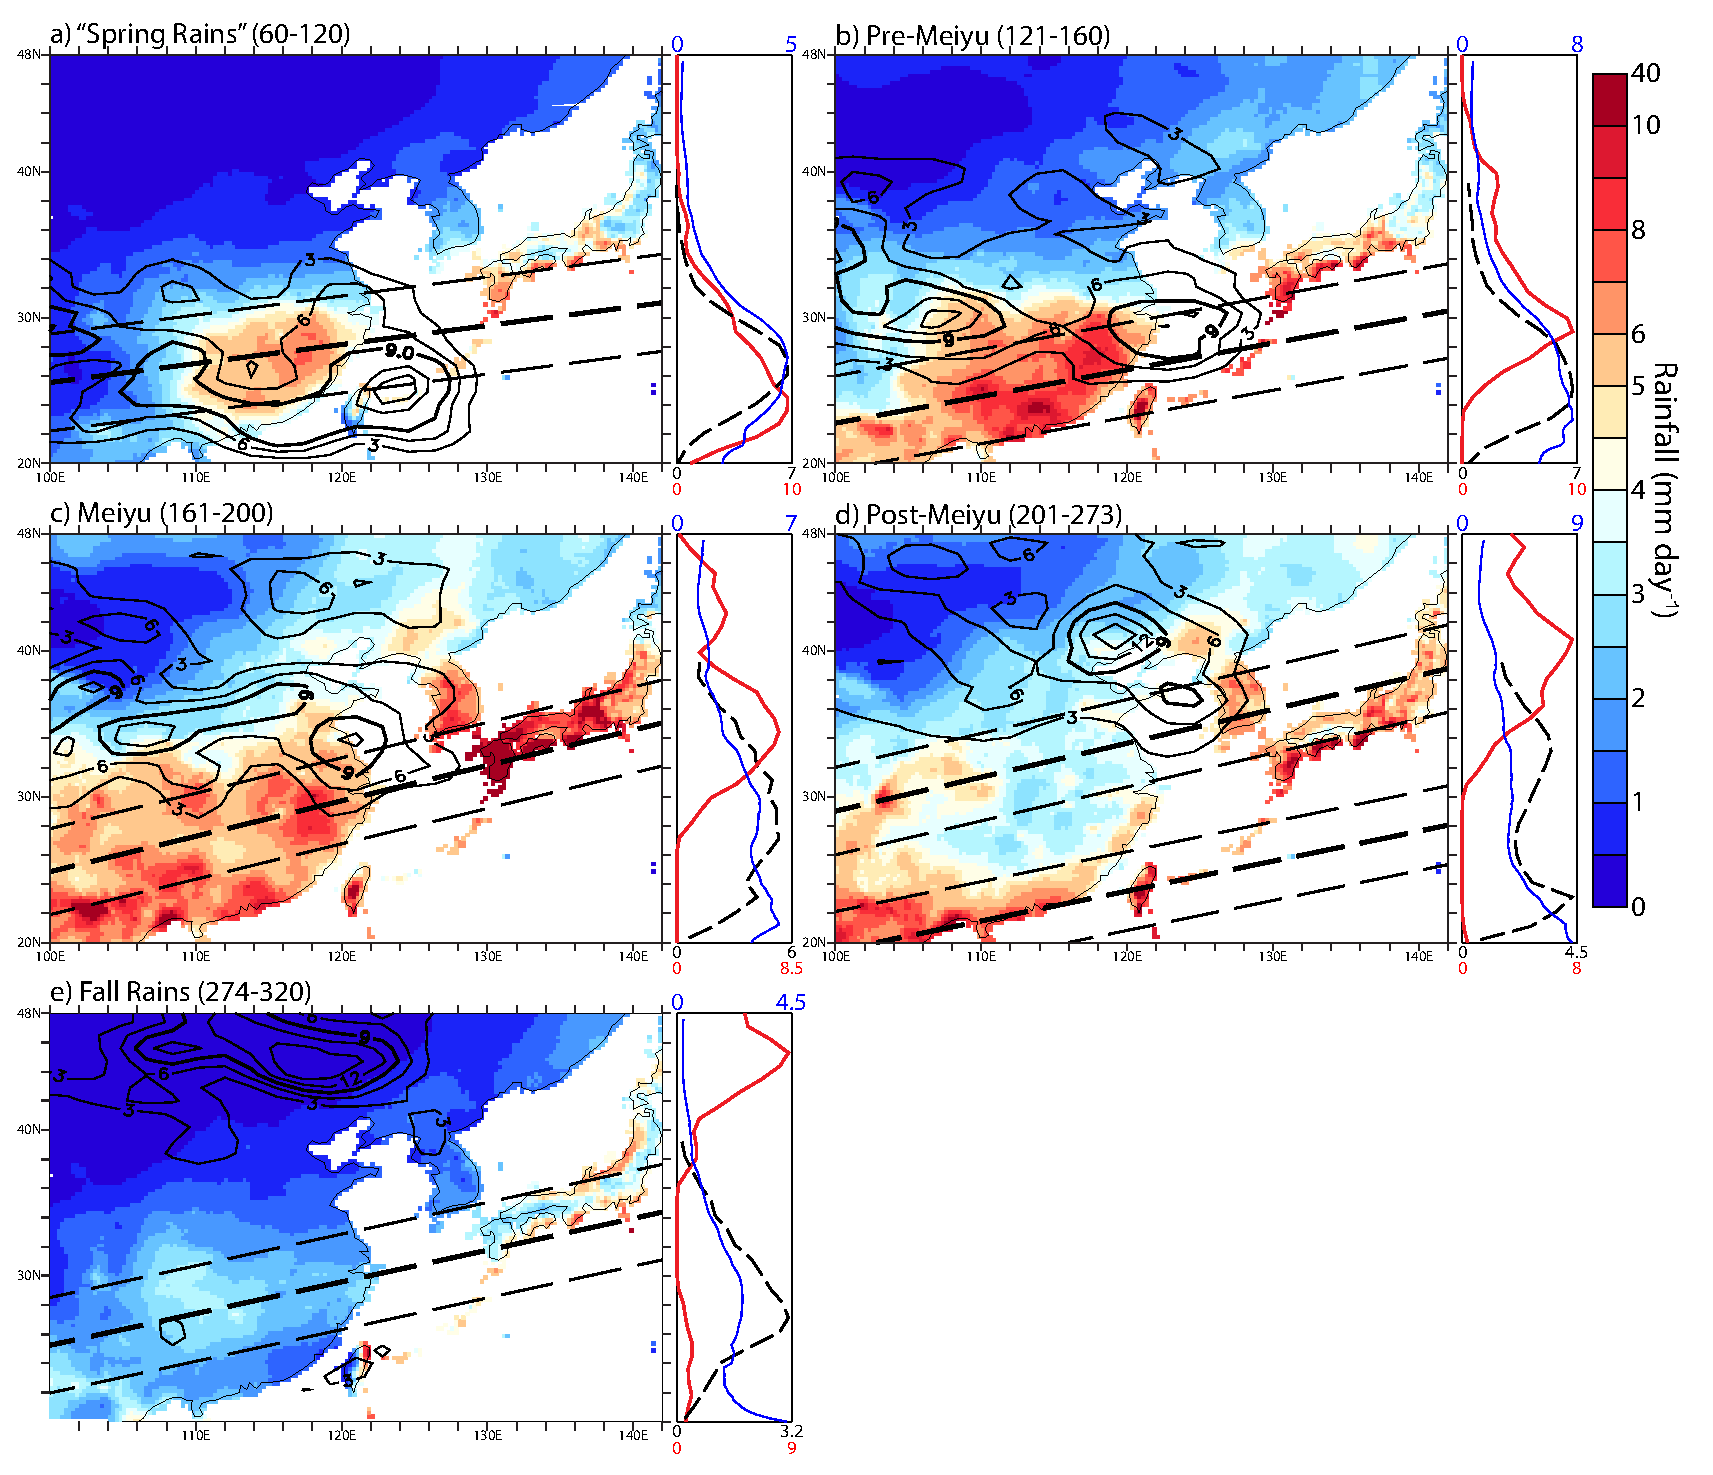
\includegraphics[width=36pc]{Figures/ch4/climo}
\caption{Climatology of East Asian rainfall stages showing rainfall (shading), jet kernel density (contours of probability density in units of $10^{-4}$) and most common rainband position during that stage. Sidebars shows, for each time period, the longitude average over 105-123$^{\circ}$E of rainfall (thin blue line, units of mm day$^{-1}$), jet kernel density (red line, units of $10^{-4}$) and rainband position (dashed black line, absolute probability in \%, 1-degree latitude smoothing). From the Pre-Meiyu to Post-Meiyu, a peak in preferred jet latitude consistently occurs 5 degrees north of a corresponding maximum in rainband frequency.}
\label{fig:climo}
\end{figure}


%% FIGURE 4.2 - 2D spatial distribution of change showing a) full year b) Pre-Meiyu and c) Post-Meiyu
\begin{figure}
\centering
\noindent\includegraphics[width=36pc]{Figures/ch4/changes_2d_jet}
\caption{a) Whole year mean rainfall change, showing the South Flood-North Drought pattern; b) Rainfall changes during the Pre-Meiyu (days 121-160) with contours of jet density change overlain; c) Same as c, but for the Post-Meiyu (days 201-273). Statistical significance at 95\%/99\% level overlain with single/double hatches. Sidebars show, for each time period, the longitude average over 105-123$^{\circ}$E of changes in rainfall (thin blue line, units of mm day$^{-1}$), jet kernel density (red line, units of $10^{-4}$) and rainband position (dashed black line, absolute probability in \%, 1-degree latitude smoothing).}
\label{fig:changes_2d}
\end{figure}

%% FIGURE 4.3 - Changes in jet mean between 1951-1979 and 1980-2007 + scatter plots of jet and rainband monthly anomalies.
\begin{figure}[htbp]
\centering
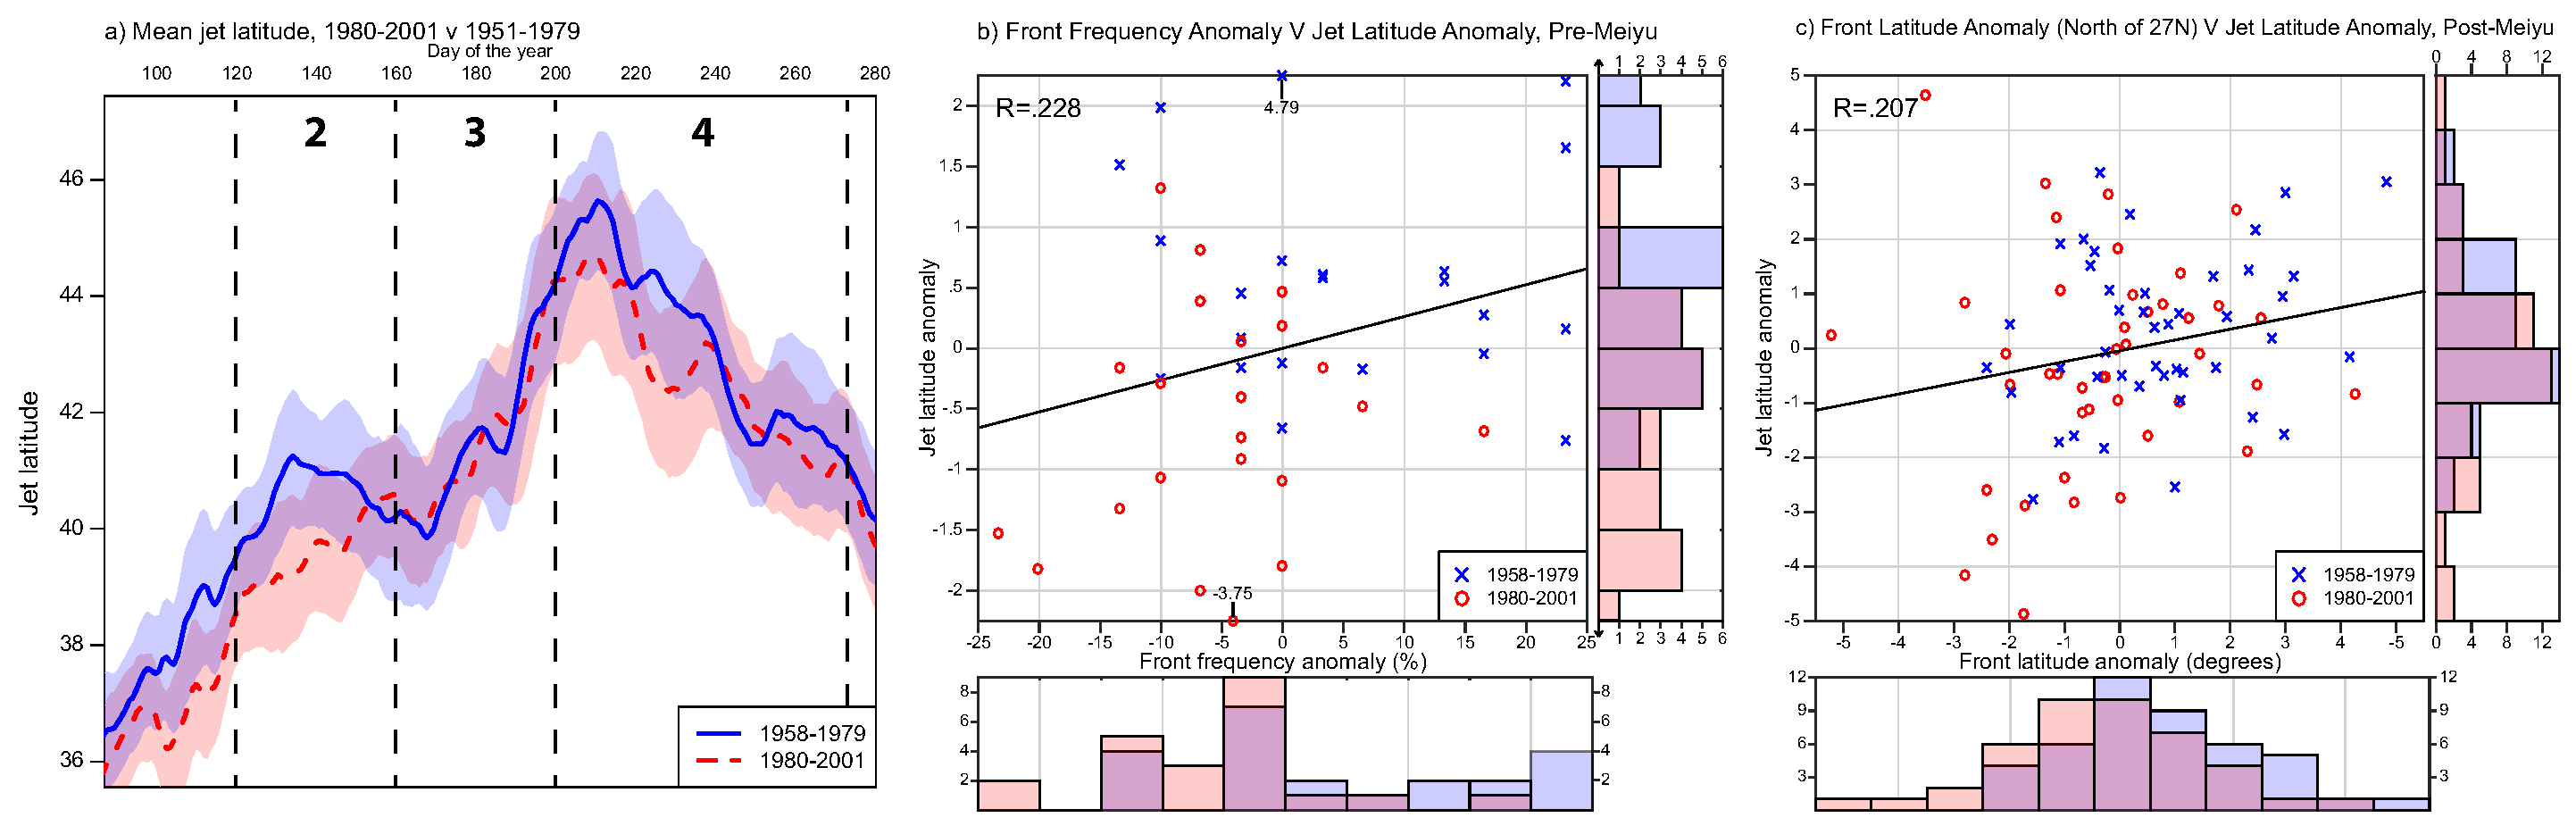
\includegraphics[width=42pc]{Figures/ch4/jet}
\caption{a) 7-day running mean latitude of the westerly jet in the region 90-130$^\circ$E for the years 1958-1979 (blue, solid) and 1980-2001 (red, dashed). Bootstrapped 95\% confidence intervals are shaded. Time periods: 2 - Pre-Meiyu; 3 - Meiyu; 4 - Post-Meiyu; b) Plot of monthly anomalies in rainband frequency versus monthly anomalies in jet latitude during days 121-150 (May) for 1958-1979 (blue X) versus 1980-2001 (red circle); c) Same as b), but showing 30-day anomalies of rainband latitudes during the Post-Meiyu (201-230 and 231-260, each set of 30 days treated as a separate point). Histograms of anomalies are also shown on the side of each figure.}
\label{fig:jet_seasonal}
\end{figure}

%% FIGURE 4.4 - Temporal autocorrelation of the jet used to demonstrate the choice of block size for averaging.
\begin{figure}[htbp]
\centering
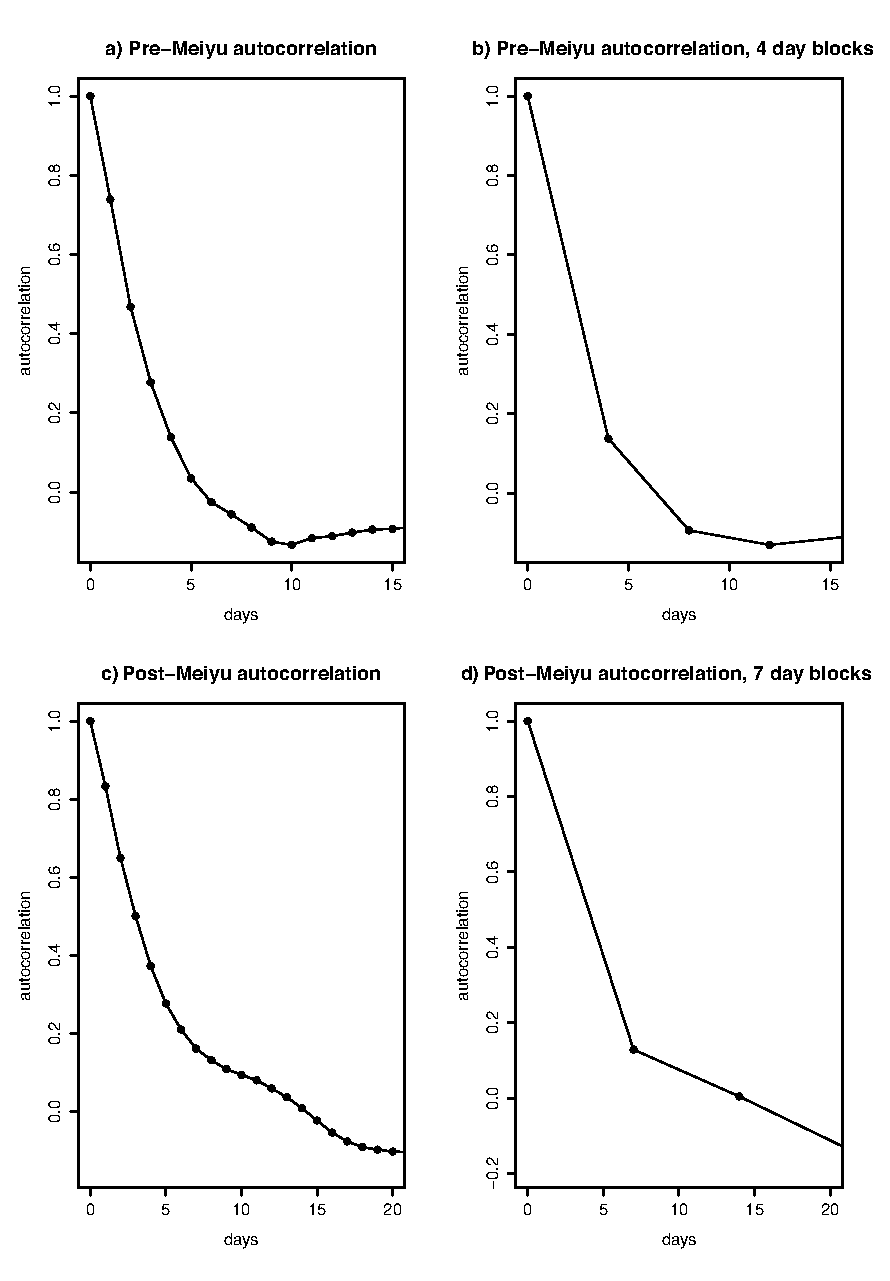
\includegraphics[width=42pc]{Figures/ch4/jet_autocorr}
\caption{The accumulation of the jet into blocks eliminates the autocorrelation from the daily mean latitude signal. During the Pre-Meiyu, mean daily jet latitude is further smoothed over 4 days (panels a and b); During the Post-Meiyu, we average over 7 days (panels c and d).}
\label{fig:jet_autocorr}
\end{figure}
